\documentclass[12pt]{book}

\usepackage{graphicx,color}
\usepackage{amssymb, amsmath, array}
\usepackage{ccicons}
%\usepackage[a4paper,top=3cm,bottom=2cm,left=2cm,right=2cm,marginparwidth=1.2cm]{geometry}
\usepackage[a4paper,top=3cm,bottom=2cm,left=3cm,right=2cm,marginparwidth=1.2cm,twoside]{geometry}
\usepackage{fancyhdr}
\usepackage{tikz}
\usetikzlibrary{shapes.geometric, arrows}
\usepackage{pgfplots}
\usepackage{caption}
\usepackage{xcolor}
\usepackage{mdframed}
\usepgfplotslibrary{fillbetween}
\pgfplotsset{compat=1.18}
\usepackage{float}

\tikzstyle{startstop} = [rectangle, rounded corners, minimum width=3cm, minimum height=1cm,text centered, draw=black, fill=red!30]
\tikzstyle{process} = [rectangle, minimum width=3cm, minimum height=1cm, text centered, draw=black, fill=orange!30]
\tikzstyle{arrow} = [thick,->,>=stealth]
\tikzstyle{box} = [rectangle, minimum width=3cm, minimum height=1cm, text centered, draw=black]

\begin{document}

% Example of title page for the projects carried out within the lasec 

% Simply include it in your mastex tex file: 
%        % Example of title page for the projects carried out within the lasec 

% Simply include it in your mastex tex file: 
%        % Example of title page for the projects carried out within the lasec 

% Simply include it in your mastex tex file: 
%        \input{cover}


% Updated March 2006 (SP)




\newcommand{\logouo}[0]{
  \begin{center}
    
\includegraphics[width=7cm]{Otago.eps}
  \end{center}
  \vspace{0.3cm}
  \hrulefill
}
\newcommand{\project}[1]{
  \begin{center}
    \large{#1}
  \end{center}
  \vspace{1cm}
}
\newcommand{\department}[1]{
  \begin{center}
    \large{#1}
  \end{center}
}
\newcommand{\supervisor}[4]{
  \begin{center}
    \begin{normalsize}{
        \bf #1}\\#2\\#3\\#4
    \end{normalsize}
  \end{center}
}
\renewcommand{\author}[1]{
  \begin{center}
    \Large{#1}
  \end{center}
  \vspace{0.5cm}
}
\renewcommand{\title}[1]{
  \vspace{3cm}
  \begin{center}
    \huge{#1}
  \end{center}
  \vspace{1.7cm}
}
\renewcommand{\date}[2]{
  \begin{center}
    \normalsize{#1 #2}
  \end{center}
  \vspace{0.5cm}
}


\thispagestyle{empty}


% begin title page
  \logouo
  
  \title{STAT115 \\
  Tutoring Materials}
  
  \author{}
  \department{Disability Information and Support (DI\&S)}
  
  \date{July}{2025}

  \begin{center}
    \begin{tabular}{cc}
      \begin{tabular}{p{6.0cm}}
        \supervisor{Tutor}{Eden Li (he/him)}{Ph.: +64 27 361 4776}{Email: eden.li@otago.ac.nz}
      \end{tabular}
    \end{tabular}
  \end{center}
 
% end title page




% Updated March 2006 (SP)




\newcommand{\logouo}[0]{
  \begin{center}
    
\includegraphics[width=7cm]{Otago.eps}
  \end{center}
  \vspace{0.3cm}
  \hrulefill
}
\newcommand{\project}[1]{
  \begin{center}
    \large{#1}
  \end{center}
  \vspace{1cm}
}
\newcommand{\department}[1]{
  \begin{center}
    \large{#1}
  \end{center}
}
\newcommand{\supervisor}[4]{
  \begin{center}
    \begin{normalsize}{
        \bf #1}\\#2\\#3\\#4
    \end{normalsize}
  \end{center}
}
\renewcommand{\author}[1]{
  \begin{center}
    \Large{#1}
  \end{center}
  \vspace{0.5cm}
}
\renewcommand{\title}[1]{
  \vspace{3cm}
  \begin{center}
    \huge{#1}
  \end{center}
  \vspace{1.7cm}
}
\renewcommand{\date}[2]{
  \begin{center}
    \normalsize{#1 #2}
  \end{center}
  \vspace{0.5cm}
}


\thispagestyle{empty}


% begin title page
  \logouo
  
  \title{STAT115 \\
  Tutoring Materials}
  
  \author{}
  \department{Disability Information and Support (DI\&S)}
  
  \date{July}{2025}

  \begin{center}
    \begin{tabular}{cc}
      \begin{tabular}{p{6.0cm}}
        \supervisor{Tutor}{Eden Li (he/him)}{Ph.: +64 27 361 4776}{Email: eden.li@otago.ac.nz}
      \end{tabular}
    \end{tabular}
  \end{center}
 
% end title page




% Updated March 2006 (SP)




\newcommand{\logouo}[0]{
  \begin{center}
    
\includegraphics[width=7cm]{Otago.eps}
  \end{center}
  \vspace{0.3cm}
  \hrulefill
}
\newcommand{\project}[1]{
  \begin{center}
    \large{#1}
  \end{center}
  \vspace{1cm}
}
\newcommand{\department}[1]{
  \begin{center}
    \large{#1}
  \end{center}
}
\newcommand{\supervisor}[4]{
  \begin{center}
    \begin{normalsize}{
        \bf #1}\\#2\\#3\\#4
    \end{normalsize}
  \end{center}
}
\renewcommand{\author}[1]{
  \begin{center}
    \Large{#1}
  \end{center}
  \vspace{0.5cm}
}
\renewcommand{\title}[1]{
  \vspace{3cm}
  \begin{center}
    \huge{#1}
  \end{center}
  \vspace{1.7cm}
}
\renewcommand{\date}[2]{
  \begin{center}
    \normalsize{#1 #2}
  \end{center}
  \vspace{0.5cm}
}


\thispagestyle{empty}


% begin title page
  \logouo
  
  \title{STAT115 \\
  Tutoring Materials}
  
  \author{}
  \department{Disability Information and Support (DI\&S)}
  
  \date{July}{2025}

  \begin{center}
    \begin{tabular}{cc}
      \begin{tabular}{p{6.0cm}}
        \supervisor{Tutor}{Eden Li (he/him)}{Ph.: +64 27 361 4776}{Email: eden.li@otago.ac.nz}
      \end{tabular}
    \end{tabular}
  \end{center}
 
% end title page



\begin{center}
	\ccbyncsa
\end{center}

%%%%%%%%%%%%%%%%%%%%%%%%%%%%%%%%%%%%%%
%%%%%%%%%%%%%%%%%%%%%%%%%%%%%%%%%%%%%%
%%%%%%%%%%%%%%%%%%%%%%%%%%%%%%%%%%%%%%
%%%%%%%%%%TERMS%%%%%%%%%%%%%
%%%%%%%%%%%%%%%%%%%%%%%%%%%%%%%%%%%%%%
%%%%%%%%%%%%%%%%%%%%%%%%%%%%%%%%%%%%%%


\newpage
\thispagestyle{empty}
\mbox{}
\newpage

\setcounter{page}{1}

\pagestyle{fancy}
\lhead{STAT110/115 Tutoring Materials}
\rhead{Terms}

\begin{itemize}
  %----------------------------------------------------------
  % Core population–sample concepts
  %----------------------------------------------------------
  \item \textbf{Population}: the entire group we want to learn about.
  \item \textbf{Sample}: the subset of that population we actually observe.
  \item \textbf{Parameter} (population quantity) vs.\ \textbf{Statistic} (sample-based estimate).

  %----------------------------------------------------------
  % Common symbols
  %----------------------------------------------------------
  \item $\mu$ - population mean \newline \quad\; $\sigma$ - population standard deviation \newline \quad\;
        $\pi$ - population proportion.
  \item $\bar{x}$ - sample mean \newline \quad\; $s$ - sample standard deviation \newline \quad\;
        $\hat{p}$ - sample proportion.

  %----------------------------------------------------------
  % Proportion / ratio / rate
  %----------------------------------------------------------
  \item \textbf{Proportion}: fraction of the (sample or population) total in a given category
        ($0 \le \hat{p} \le 1$).
  \item \textbf{Ratio}: numerator and denominator have the \emph{same} units (e.g.\ waist/hip).
  \item \textbf{Rate}: numerator and denominator have \emph{different} units
        (e.g.\ km per hour; cases per 1,000 person-years).

  %----------------------------------------------------------
  % Random variables
  %----------------------------------------------------------
  \item \textbf{Random variable} $X$: an unknown quantity described by a probability distribution.
  \item \textbf{Observed (realised) value} $x$: the concrete outcome recorded in the data.

  %----------------------------------------------------------
  % Variable types
  %----------------------------------------------------------
  \item \textbf{Variable types}
        \begin{itemize}
          \item \textbf{Quantitative}
                \begin{itemize}
                  \item \emph{Continuous}: can take any value on an interval
                        (e.g.\ height, blood pressure).
                  \item \emph{Discrete}: isolated values, usually counts
                        (e.g.\ number of GP visits).
                \end{itemize}
          \item \textbf{Categorical}
                \begin{itemize}
                  \item \emph{Binary / dichotomous}: two categories
                        (e.g.\ pass vs.\ fail).
                  \item \emph{Nominal}: $\ge 2$ unordered categories
                        (e.g.\ blood type A/B/O/AB).
                  \item \emph{Ordinal}: ordered categories
                        (e.g.\ pain score 0–10, Likert scale).
                \end{itemize}
        \end{itemize}

  %----------------------------------------------------------
  % Censored data – will be revisited in survival analysis weeks
  %----------------------------------------------------------
  \item \textbf{Censored data}
        \begin{itemize}
          \item \textbf{Right-censored}: true value is \emph{greater} than a known limit  
                (e.g.\ patient still alive at study end; age $>90$).
          \item \textbf{Left-censored}: true value is \emph{smaller} than a detection limit  
                (e.g.\ viral load $<10$ copies/mL).
          \item \textbf{Interval-censored}: true value lies between two known bounds  
                (e.g.\ infection occurs between two clinic visits two years apart).
        \end{itemize}
\end{itemize}

%%%%%%%%%%%%%%%%%%%%%%%%%%%%%%%%%%%%%%
%%%%%%%% R (quick-reference) %%%%%%%%%
%%%%%%%%%%%%%%%%%%%%%%%%%%%%%%%%%%%%%%

\newpage
\pagestyle{fancy}
\lhead{STAT110/115 Tutoring Materials}
\rhead{R Functions}

\begin{itemize}

% ============================================================
% 0. Getting started & help
% ============================================================
\item \textbf{Getting help \& packages}
  \begin{itemize}
    \item Install once: \texttt{install.packages("tidyverse")}  \hfill\emph{(data wrangling / plots)}
    \item Load every session: \texttt{library(tidyverse)}
    \item Function help: \texttt{?lm}, worked example: \texttt{example(t.test)}
  \end{itemize}

% ============================================================
% 1. Data import & quick exploration
% ============================================================
\item \textbf{Data import \& quick checks}
  \begin{itemize}
    \item CSV: \texttt{df <- read.csv("myfile.csv", stringsAsFactors = FALSE)}
    \item Peek: \texttt{head(df)}, \texttt{str(df)}, \texttt{summary(df)}
    \item Subset rows: \texttt{dplyr::filter(df, Group == "A")}
  \end{itemize}

% ============================================================
% 2. Descriptive statistics
% ============================================================
\item \textbf{Descriptive statistics}
  \begin{itemize}
    \item Centre: \texttt{mean(x)}, \texttt{median(x)}
    \item Spread: \texttt{sd(x)}, \texttt{IQR(x)}, \texttt{var(x)}
    \item Always add \texttt{na.rm = TRUE} if missing values exist
    \item Correlation: \texttt{cor(x, y)} (number) \; | \;
          \texttt{cor.test(x, y)} (CI + $p$)
  \end{itemize}

% ============================================================
% 3. Graphics (base R)
% ============================================================
\item \textbf{Base R graphics}
  \begin{itemize}
    \item Histogram: \texttt{hist(x, breaks = 20, main = "Histogram")}
    \item Scatterplot: \texttt{plot(df$X, df$Y, main = "Scatterplot")}
  \end{itemize}

% ============================================================
% 4. Probability distributions
% ============================================================
\item \textbf{Key distribution helpers}

  \textbf{Normal} $Z\sim N(0,1)$
  \begin{itemize}
    \item Density: \texttt{dnorm(z)}
    \item Tail area: \texttt{pnorm(q)} ($=P(Z\le q)$)
    \item Quantile: \texttt{qnorm(p)}
    \item Random draw: \texttt{rnorm(n)}
  \end{itemize}

  \textbf{$t$-dist} $T_\nu$
  \begin{itemize}
    \item \texttt{dt(x, df)}, \texttt{pt(t, df)}, \texttt{qt(p, df)}, \texttt{rt(n, df)}
  \end{itemize}

  \textbf{Binomial} $X\sim\mathrm{Bin}(n,\pi)$
  \begin{itemize}
    \item Point prob: \texttt{dbinom(x, n, pi)}
    \item Cumulative: \texttt{pbinom(q, n, pi)}
    \item Quantile: \texttt{qbinom(p, n, pi)}
    \item Random draw: \texttt{rbinom(N, n, pi)}
  \end{itemize}

  \textbf{$\chi^2$ \& F}
  \begin{itemize}
    \item $\chi^2$ tail: \texttt{pchisq(q, df, lower.tail = FALSE)}
    \item Critical $\chi^2$: \texttt{qchisq(0.95, df)}
    \item F tail: \texttt{pf(F, df1, df2, lower.tail = FALSE)}
    \item Critical F: \texttt{qf(0.95, df1, df2)}
  \end{itemize}

% ============================================================
% 5. Confidence intervals & t-tests
% ============================================================
\item \textbf{Confidence intervals \& $t$-tests}
  \begin{itemize}
    \item One-sample mean: \texttt{t.test(x, mu = mu0)}
    \item Two independent groups: \texttt{t.test(y ~ g, data = df)}  
          (\texttt{var.equal = TRUE} for pooled)
    \item Paired: \texttt{t.test(before, after, paired = TRUE)}
    \item Exact one-prop CI / test: \texttt{binom.test(x, n)}
  \end{itemize}

% ============================================================
% 6. Tables & tests for proportions
% ============================================================
\item \textbf{Two-way tables \& $\chi^2$ / Fisher}
  \begin{itemize}
    \item Build: \texttt{tab <- table(df$A, df$B)}; totals: \texttt{addmargins(tab)}
    \item $\chi^2$ test: \texttt{chisq.test(tab)}
    \item Small expected counts? use \texttt{fisher.test(tab)}
  \end{itemize}
\item \textbf{Proportion tests}
  \begin{itemize}
    \item One / two props (large $n$): \texttt{prop.test(x = c(18,12), n = c(30,30))}
  \end{itemize}

% ============================================================
% 7. Linear models & ANOVA
% ============================================================
\item \textbf{Simple \& multiple linear regression}
  \begin{itemize}
    \item Fit: \texttt{fit <- lm(Y ~ X1 + X2, data = df)}
    \item Inspect: \texttt{summary(fit)}; 95\% CI: \texttt{confint(fit)}
    \item Predict: \texttt{predict(fit, newdata = data.frame(X1 = 10, X2 = 5),
          interval = "confidence")}
  \end{itemize}

\item \textbf{Logistic regression (STAT115 Weeks 10-11)}
  \begin{itemize}
    \item Binary outcome: \texttt{logit <- glm(case ~ age + sex,\; family = binomial,\; data = df)}
    \item Odds ratios: \texttt{exp(coef(logit))}; CI: \texttt{exp(confint(logit))}
  \end{itemize}

\item \textbf{One-way ANOVA \& multiple comparisons}
  \begin{itemize}
    \item Overall model: \texttt{a1 <- aov(y ~ group, data = df)}
    \item Summary table: \texttt{summary(a1)}
    \item Pairwise Tukey: \texttt{TukeyHSD(a1)}  \hfill\emph{(controls family-wise error)}
  \end{itemize}

% ============================================================
% 8. Simulation helpers
% ============================================================
\item \textbf{Simulation snippets}
  \begin{itemize}
    \item Reproducibility: \texttt{set.seed(123)}
    \item 1\,000 $N(0,1)$ draws: \texttt{x <- rnorm(1000)}
    \item Central-limit-theorem demo:  
          \texttt{ybar <- replicate(1e4, mean(rnorm(50)))} \hfill\emph{(hist to visualise)}
  \end{itemize}

% ============================================================
% 9. House-keeping
% ============================================================
\item \textbf{Workspace utilities}
  \begin{itemize}
    \item Clear memory: \texttt{rm(list = ls())}
    \item Save history: \texttt{savehistory("my\_hist.Rhistory")}
  \end{itemize}

\end{itemize}


%%%%%%%%%%%%%%%%%%%%%%%%%%%%%%%%%%%%%%
%%%%%%%%% PROBABILITY (Week 2) %%%%%%%
%%%%%%%%%%%%%%%%%%%%%%%%%%%%%%%%%%%%%%

\newpage
\pagestyle{fancy}
\lhead{STAT110/115 Tutoring Materials}
\rhead{Probability}

\begin{itemize}

% -----------------------------------------------------------
% 0. What do we mean by “probability”?
% -----------------------------------------------------------
\item \textbf{Subjective probability} – a personal degree of belief  
      (e.g.\ “I’m 80 \% sure it will rain tomorrow”).
\item \textbf{Objective / long–run probability} – the proportion of times an event occurs
      in a very large number of identical trials (e.g.\ coin toss heads $\approx 0.5$).

% -----------------------------------------------------------
% 1. Sample space \& events
% -----------------------------------------------------------
\item \textbf{Sample space} $S$ – all possible outcomes of an experiment  
      (fair die: $S=\{1,2,3,4,5,6\}$).
\item \textbf{Event} $A$ – a subset of $S$ (e.g.\ “even number” = $\{2,4,6\}$).

% -----------------------------------------------------------
% 2. Basic rules
% -----------------------------------------------------------
\item \textbf{Complement}:\quad $P(A)+P(\overline{A}) = 1$.
\item \textbf{Addition rule} (two events):\quad
      $P(A\cup B)=P(A)+P(B)-P(A\cap B)$.
\item \textbf{Multiplication rule / conditional prob.}:\quad
      $P(A\cap B)=P(A)\,P(B\,|\,A)$.

% -----------------------------------------------------------
% 3. Independence
% -----------------------------------------------------------
\item \textbf{Independent events} – knowing one tells us nothing about the other.
      Equivalent checks:  
      \[
        P(A\cap B)=P(A)\,P(B)\quad\Longleftrightarrow\quad
        P(B)=P(B\,|\,A)\quad\Longleftrightarrow\quad
        P(A)=P(A\,|\,B).
      \]

% -----------------------------------------------------------
% 4. Diagnostic-test notation (STAT115 focus)
% -----------------------------------------------------------
\begin{itemize}
  \item $A$ = person \emph{has} the disease, $\overline{A}$ = person \emph{does not}.
  \item $B$ = test is \emph{positive}, $\overline{B}$ = test is \emph{negative}.
\end{itemize}

\begin{tabular}{@{}ll@{}}
\textbf{Sensitivity} & $P(B\,|\,A)$          – probability the test detects the disease.\\
\textbf{Specificity} & $P(\overline{B}\,|\,\overline{A})$ – probability a healthy person tests negative.\\
\textbf{False-positive rate} & $1-\text{specificity}=P(B\,|\,\overline{A})$.\\
\textbf{Positive Predictive Value (PPV)} & $P(A\,|\,B)$ – “If the test is positive, how likely is disease?”\\
\textbf{Negative Predictive Value (NPV)} & $P(\overline{A}\,|\,\overline{B})$.\\
\end{tabular}

% -----------------------------------------------------------
% 5. Bayes’ theorem (links PPV/NPV to prevalence)
% -----------------------------------------------------------
\[
  P(A\,|\,B)=\frac{P(B\,|\,A)\,P(A)}{P(B\,|\,A)P(A)+P(B\,|\,\overline{A})P(\overline{A})}.
\]
\emph{Tip:} Low disease prevalence ($\downarrow$) $\Rightarrow$ PPV tends to be low even when sensitivity and specificity are high.

% -----------------------------------------------------------
% 6. Two-by-two table quick check
% -----------------------------------------------------------
\[
\begin{array}{c|cc|c}
           & \text{Disease }A & \text{No disease }\overline{A} & \text{Total} \\ \hline
\text{Test + }B     & a & b & a+b \\
\text{Test – }\overline{B} & c & d & c+d \\ \hline
\text{Total} & a+c & b+d & n
\end{array}
\]
\begin{itemize}
  \item Sensitivity $=a/(a+c)$,\; Specificity $=d/(b+d)$.
  \item PPV $=a/(a+b)$,\; NPV $=d/(c+d)$.
\end{itemize}

\end{itemize}


%%%%%%%%%%%%%%%%%%%%%%%%%%%%%%%%%%%%%%
%%%%%%%%%%%%%%%%%%%%%%%%%%%%%%%%%%%%%%
%%%%%%%%%%%%%%%%%%%%%%%%%%%%%%%%%%%%%%
%%%%%%%%CONTINGENCY TABLE%%%%%%%%%
%%%%%%%%%%%%%%%%%%%%%%%%%%%%%%%%%%%%%%
%%%%%%%%%%%%%%%%%%%%%%%%%%%%%%%%%%%%%%
%%%%%%%%%%%%%%%%%%%%%%%%%%%%%%%%%%%%%%

\newpage

\pagestyle{fancy}
\lhead{STAT110/115 Tutoring Materials}
\rhead{Contingency Table}

\begin{itemize}
\item \textbf{Relative Risk (RR)}: Ratio of two probabilities. RR gives the risk of an outcome relative to "exposure". It is calculated as the ratio of the risk of an outcome for an exposed and an unexposed group. $$RR = \frac{a/(a+b)}{c/(c+d)}$$
Meaning of the RR value: RR = 1 there is no association between outcome and exposure (e.g. rugby position and injury). RR < 1 first row happens less likely than the second row. RR > 1 first row happens more likely than the second row.
\item \textbf{Risk Difference (RD)}: Difference between two probabilities. The RD is given by the difference in the risk for the two groups. $$RD = \frac{a}{a + b} - \frac{c}{c + d}$$
\item \textbf{Odds Ratio (OR)}: Ratio of two odds. The OR compares the odds of an outcome for two groups. Ratio of the odds of the outcome for the exposed group to that for the unexposed group. $$OR = \frac{a/b}{c/d} = \frac{ad}{bc}$$. There is no mathematical distinction between exposure and outcome variables -> makes it particularly useful for quantifying associations between binary variables where there is no "direction" e.g. alcohol consumption (Yes/No) and smoking (Yes/No).
\item \textbf{Confidence Interval for Difference Between Two Proportions}: $$p1 = \frac{a}{r1}$$, $$p2 = \frac{c}{r2}$$, $$(p_1 - p_2) \pm Z_{(1 - \frac{\alpha}{2})} \sqrt{\frac{p_1(1-p_1)}{n_1} + \frac{p_2(1-p_2)}{n_2}}$$

\item \textbf{Steps to Calculate the Confidence Interval for Relative Risk}:
    \begin{itemize}
    \item Get the RR value.
    \item Get the ln(RR).
    \item Calculate the SE of ln(RR) (with formula).
    \item Calculate the CI for ln(RR) (with formula).
    \item Calculate the CI for RR (exp() function).
    \end{itemize}
\item \textbf{Standard error for Confidence interval for relative risk:}$$S_{ln}(RR) = \sqrt{\frac{1}{a} - \frac{1}{r_1} + \frac{1}{c} - \frac{1}{r_2}}$$
\item \textbf{Key formula for Confidence interval for relative risk:}$$\ln(RR) \pm Z_{(1-\frac{\alpha}{2})} \cdot S_{\ln(RR)}$$
\item \textbf{Steps to Calculate the Confidence Interval for Odds Ratio}:
    \begin{itemize}
    \item Get the OR value.
    \item Get the ln(OR).
    \item Calculate the SE of ln(OR) (with formula).
    \item Calculate the CI for ln(OR) (with formula).
    \item Calculate the CI for OR (exp() function).
    \end{itemize}
\item \textbf{Standard error for Confidence interval for Odds Ratio:} $$S_{\ln(OR)} = \sqrt{\frac{1}{a} + \frac{1}{b} + \frac{1}{c} + \frac{1}{d}}$$
\item \textbf{The meaning for range of CI:}
\begin{figure} [H]
\centering
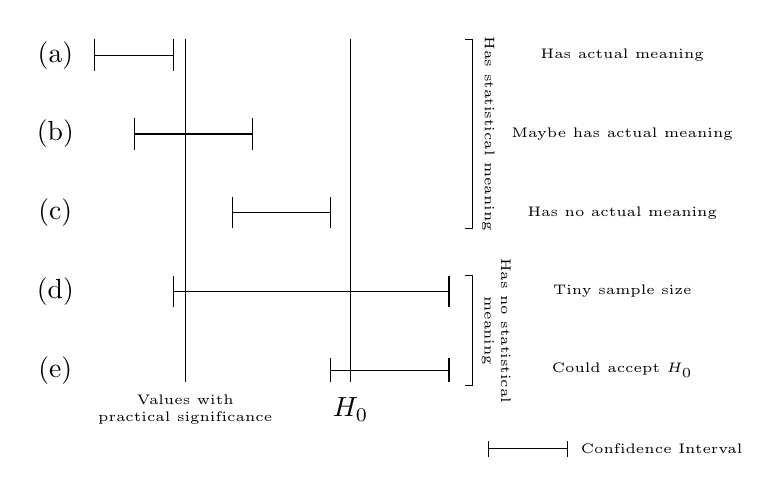
\begin{tikzpicture}
% Horizontal lines with error bars
\draw (0,5) -- (1,5); % Line a
\draw (0, 4.8) -- (0, 5.2); % Error bar for line a
\draw (1, 4.8) -- (1, 5.2); % Error bar for line a

\draw (0.5,4) -- (2,4); % Line b
\draw (0.5, 3.8) -- (0.5, 4.2); % Error bar for line b
\draw (2, 3.8) -- (2, 4.2); % Error bar for line b

\draw (1.75,3) -- (3,3); % Line c
\draw (1.75, 2.8) -- (1.75, 3.2); % Error bar for line c
\draw (3, 2.8) -- (3, 3.2); % Error bar for line c

\draw (1,2) -- (4.5,2); % Line d
\draw (1, 1.8) -- (1, 2.2); % Error bar for line d
\draw (4.5, 1.8) -- (4.5, 2.2); % Error bar for line d

\draw (3,1) -- (4.5,1); % Line e
\draw (3, 0.85) -- (3, 1.15); % Error bar for line e
\draw (4.5, 0.85) -- (4.5, 1.15); % Error bar for line e

\draw (1.15, 0.85) -- (1.15, 5.2); % first bar
\draw (3.25, 0.85) -- (3.25, 5.2); % second bar

% Labels for horizontal lines
\node at (-0.5,5) {(a)};
\node at (-0.5,4) {(b)};
\node at (-0.5,3) {(c)};
\node at (-0.5,2) {(d)};
\node at (-0.5,1) {(e)};

\node [font=\tiny, align=left] at (6.7, 5) {Has actual meaning};
\node [font=\tiny, align=left] at (6.7, 4) {Maybe has actual meaning};
\node [font=\tiny, align=left] at (6.7, 3) {Has no actual meaning};
\node [font=\tiny, align=left] at (6.7, 2) {Tiny sample size};
\node [font=\tiny, align=left] at (6.7, 1) {Could accept $H_0$};

% Vertical text on left
\node[rotate=270, font=\tiny] at (5,4) {Has statistical meaning};

\draw (4.8, 5.2) -- (4.8,2.8);
\draw (4.7, 2.8) -- (4.8,2.8);
\draw (4.7, 5.2) -- (4.8,5.2);

\node[rotate=270, font=\tiny, align=center] at (5.1,1.5) {Has no statistical \\ meaning};
\draw (4.8, 2.2) -- (4.8,0.8);
\draw (4.7, 0.8) -- (4.8,0.8);
\draw (4.7, 2.2) -- (4.8,2.2);


\draw (5,0) -- (6,0); 
\draw (5, -0.1) -- (5, 0.1);
\draw (6, -0.1) -- (6, 0.1); 
\node [font=\tiny, align=left] at (7.2, 0) {Confidence Interval};

% Text below the diagram
\node [font=\tiny, align=center] at (1.15, 0.5) {Values with \\ practical significance};
\node [align=center] at (3.25, 0.5) {$H_0$};

\end{tikzpicture}
\end{figure}
\item \textbf{Risk Difference in Terms of the Number of Cases Per x People}: To get the risk difference in terms of the number of cases per x people, we need to multiply this answer by x. For example, express your answer in terms of the extra number of cases of cancer among 1000 people who eat red or processed meat four or more times per week.  $$\frac{2341}{191678}-\frac{277}{68601}=0.008175$$
To get the risk difference in terms of the number of cases per 1000 people, we need to multiply this answer by 1000. $$RD = \left(\frac{2341}{191678}-\frac{277}{68601}\right)*1000=8.175$$
\end{itemize}

%%%%%%%%%%%%%%%%%%%%%%%%%%%%%%%%%%%%%%
%%%%%%%%%%%%%%%%%%%%%%%%%%%%%%%%%%%%%%
%%%%%%%%%%%%%%%%%%%%%%%%%%%%%%%%%%%%%%
%%%%%%%%STUDY DESIGN%%%%%%%%%
%%%%%%%%%%%%%%%%%%%%%%%%%%%%%%%%%%%%%%
%%%%%%%%%%%%%%%%%%%%%%%%%%%%%%%%%%%%%%
%%%%%%%%%%%%%%%%%%%%%%%%%%%%%%%%%%%%%%
\newpage

\pagestyle{fancy}
\lhead{STAT110/115 Tutoring Materials}
\rhead{Study Design}

\begin{itemize}
\item \textbf{Purpose of Analytic Studies}: To test hypotheses (quantify population). For example, do government subsidy programs impact the profitability of fisheries? Does IT investment impact productivity in industry? Does a Mediterranean diet impact life expectancy?
\item \textbf{Function of Replication}: To allow us to separate out true effects from chance effects.
\item \textbf{Function of Control}: Provides context for evaluating the effect of interest.
\item \textbf{Descriptive Studies}: The characteristics of people with a disease (person; place; time); lifestyle patterns in a population; attitudes to health care.
\item \textbf{Well-defined and Not Well-defined Population}:
    \begin{itemize}
    \item Well-defined: The collection of words in poems by W. B. Yeats. All patients diagnosed with colorectal cancer in New Zealand in 2015.
    \item Not well-defined: The population of New Zealand. Right now? Past? Future?(Time). Target population for a particular cancer treatment. Which type/stage of cancer? Existing or future patients(time)? Over a certain age? On other medications?
    \end{itemize}
\item \textbf{Traits of Random Sampling}: Known-chance, Equal-chance. If doesn't have those traits, define the sample has representative or not.
\item \textbf{Sampling Frame Definition}: List of all eligible sampling units from which the sample will be drawn. For example, to draw 200 out of 10,000 employees to form a sample, the roster of 10,000 employees, is the sampling frame. May be sourced from census, company data base or other secondary data. Completeness may be an issue when sourcing Sampling Frame. Sometimes need to use/combine multiple sample frames. Non-probability sampling techniques don't require a sampling frame.
\item \textbf{Sources of Error for Sample Mean}:

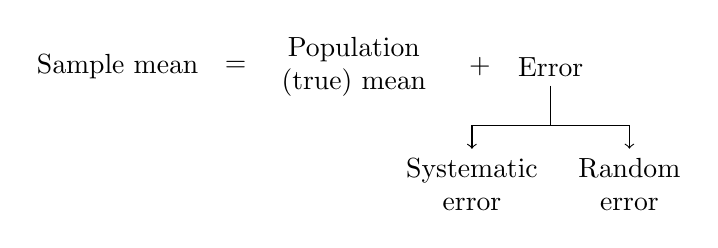
\begin{tikzpicture}
\node (samplemean) at (0,0) {Sample mean};
\node (equals) at (1.5,0) {=};
\node [align=center](populationmean) at (3,0) {Population \\ (true) mean};
\node (plus) at (4.6,0) {+};

\node (error) at (5.5,0) {Error};

\node[below of=error, align=center, xshift=-1cm, yshift=-0.5cm] (systematicerror) {Systematic \\ error};
\node[right of=systematicerror, align=center, xshift=1cm] (randomerror) {Random \\ error};

\draw[->] (error.south) -- ++(0,-0.5)-|  node[near start,below] {}(systematicerror.north);
\draw[->] 	(error.south)-- ++(0,-0.5)-| node[near start,below] {}(randomerror.north);
\end{tikzpicture}

    \begin{itemize}
    \item \textbf{Random Error}: Due to natural variability. Increasing the sample size will reduce the random fluctuations in the sample mean. Statistical methods allow us to quantify the influence of random error on our estimate.
    \item \textbf{Systematic Error in a Descriptive Study (Bias)}: Due to aspects of the design or conduct of the study which systematically distort the results. Occurs if a sample is not representative of the population (Selection bias). Occurs if the information collected from the sample members is incorrect (Information bias). Cannot be reduced by increasing the sample size.
    \end{itemize}
\item \textbf{Probability Sampling}: We want our sampling frame to match the population of interest and provide a way to draw a sample. Probability sampling is important because it helps to justify the statistical models. For a finite population of size N draw a sample of size n such that each possible sample has the same probability of being selected.
\item \textbf{Key Characteristic of Probability Sampling}: The key characteristic is that we know the probability of being selected for everyone in the sample frame.
\item \textbf{Simplest Form of Probability Sampling}: Simple random sampling.
\item \textbf{Types of Probability Sampling}: Simple random sampling, stratified random sampling, cluster sampling.
\item \textbf{Traits of Simple Random Sampling}: Same chance of selection (e.g., Lotto).
\item \textbf{Advantages of Stratified Sampling}: More precise estimate than for the same sample size from a simple random sample. Can take different-sized samples from different strata (a device for reducing overall variability). Useful if you are interested in the results for each stratum, and some of the strata are small. Example: colon cancer treatment, samples of colon cancer patients, stratified by ethnicity.
\item \textbf{Types of Stratified Sampling}: Proportionate stratified sample, disproportionate stratified sample (equal number from each stratum).
\item \textbf{Cluster Sampling}: The population may be composed of similar and naturally occurring groups. Dividing the population into a group/cluster (then selecting a sample from each cluster).
\item \textbf{Types of Cluster Sampling}: One-stage, two-stage. Pros and cons for two-stage cluster sampling: reduce cost \& time, less precise.
\item \textbf{Experimental Studies}: The researcher manipulates the conditions (intervenes in a natural process) and records the results. The aim is to control all other factors to isolate the effects of the intervention. Best way to study causation. Why randomisation? Randomisation can be used to ensure that the effects of unmeasured factors are equalised across the intervention and control groups. Why NOT experimental studies? Ethical problems.
\item \textbf{Observational Studies}: The investigator does not intervene, simply observes a naturally occurring process, and collects information. The idea is to get as close as possible to the information that would have been obtained if the experimental study could have been done. Cons: We can't know the confounding factors.
\item \textbf{Case Control Study}: Outcome trace back to reason.
\item \textbf{Traits of Randomised Controlled Trial (RCT)}: 
	\begin{itemize}
	\item Is considered the "gold standard" analytic study.
	\item \textbf{Randomisation} - or random allocation- is used to create two comparable groups, one that will have the placebo treatment and the other the experimental treatment. At the end of follow-up any difference between the groups can be attributed to the difference in treatment.
	\item \textbf{Control group} - is used to isolate the effects of the intervention.
	\end{itemize}
\item \textbf{What is blinding?}: Blinding refers to not knowing whether the participant is in the intervention or the control group. Several people may be blinded to the allocation including the participants, the people caring for patients, the people measuring outcomes, and the lead researcher.
\item \textbf{Pros and cons for RCT}
    \begin{itemize}
    \item Advantages: Experiment - the best way to test a hypothesis. If the trial is well conducted, differences in outcome can be attributed to the intervention.
    \item Disadvantages: May not be ethical or feasible.
    \end{itemize}
\item \textbf{Example cohort study}: British doctors and smoking. Aim: to investigate the relationship between smoking and lung cancer.
\item \textbf{Pros and cons for cohort study}:
    \begin{itemize}
    \item Pros: Clear chronological order from reason to outcome. Can evaluate the relationship between multiple results and factor(s).
    \item Cons: Large time consumption. Bias affects. Small sample size.
    \end{itemize}
\item \textbf{Characteristics of a case-control study}: Generally carried out to test hypotheses. Participants are chosen on the basis of their outcome status: a group with the outcome (cases) and a group without (controls). Information is collected from people with and without outcomes about exposures that occurred in the past (retrospective). i.e. in general before disease was diagnosed.
\item \textbf{Pros and cons for Case-control study}:
    \begin{itemize}
    \item Advantages: Relatively quick. Smaller than cohort studies, particularly for rare outcomes. Can examine the effects of multiple exposures.
    \item Disadvantages: Events have already occurred, so the potential for bias is higher. It is very hard (if not impossible) to remove all the effects of confounding.
    \end{itemize}
\item \textbf{Sources of error in analytic studies}

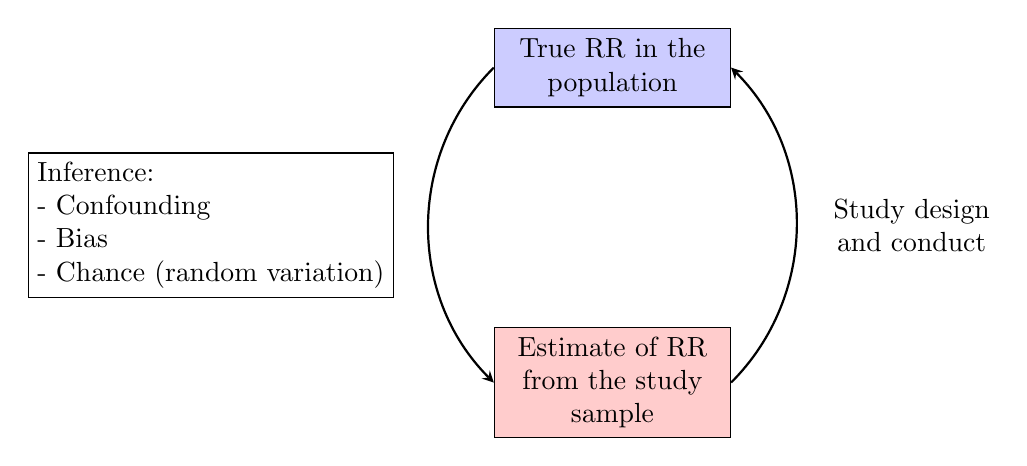
\begin{tikzpicture}[node distance=2cm]
% Nodes
\node (trueRR) [process, align=center, fill=blue!20] {True RR in the \\ population};
\node (estimateRR) [process, align=center, fill=red!20, below of=trueRR, yshift=-2cm] {Estimate of RR \\ from the study \\ sample};
\node (inference) [box, align=left, left of=trueRR, xshift=-3.1cm, yshift=-2cm] {Inference: \\ - Confounding \\ - Bias \\ - Chance (random variation)};
\node (studyDesign) [right of=trueRR, align=center, xshift=1.8cm, yshift=-2cm] {Study design \\ and conduct};
% Arrows
\draw [arrow] (trueRR.west) to [bend right=45] (estimateRR.west);
\draw [arrow] (estimateRR.east) to [bend right=45] (trueRR.east);
\end{tikzpicture}

\item \textbf{What is Confounding?}: Confounding is a distortion of the association between exposure and outcome caused by the presence of a third factor. A confounder is a variable which causes this distortion.
\item \textbf{A variable must be both ( ) to become a confounder}:
    \begin{itemize}
    \item associated with the exposure (independent of outcome);
    \item and associated with the outcome (independent of exposure).
    \end{itemize}
\item \textbf{Bias in an analytic study}:
    \begin{itemize}
    \item \textbf{Selection bias}: arising from the way participants are selected for inclusion in the study. In an analytic study, selection bias occurs if the selection processes cause a systematic difference between the groups of participants selected for the study. Prospective analytic studies rarely obtain participants through random sampling from a population. The issue of representativeness must be considered, but for analytic studies we consider it a generalisability issue rather than bias.
    \item \textbf{Information bias}: arising from the way study information is obtained, interpreted and recorded. In an analytic study, information bias is a particular problem if there are systematic differences in the information obtained from groups under comparison in the study. Information bias may be introduced by the observer, the study individual (respondent), instruments used to collect the data (e.g., badly-designed questionnaire), or missing measurements (e.g., from loss to follow-up in a prospective study).
    \end{itemize}
\item \textbf{RCT, Cohort study, Case-control study}:
    \begin{itemize}
    \item \textbf{Randomised controlled trial}: Analytic, experimental, prospective.
    \item \textbf{Cohort study}: Analytic, observational, usually prospective.
    \item \textbf{Case-control study}: Analytic, observational, retrospective.
    \end{itemize}
\item \textbf{Summary for the classification}:

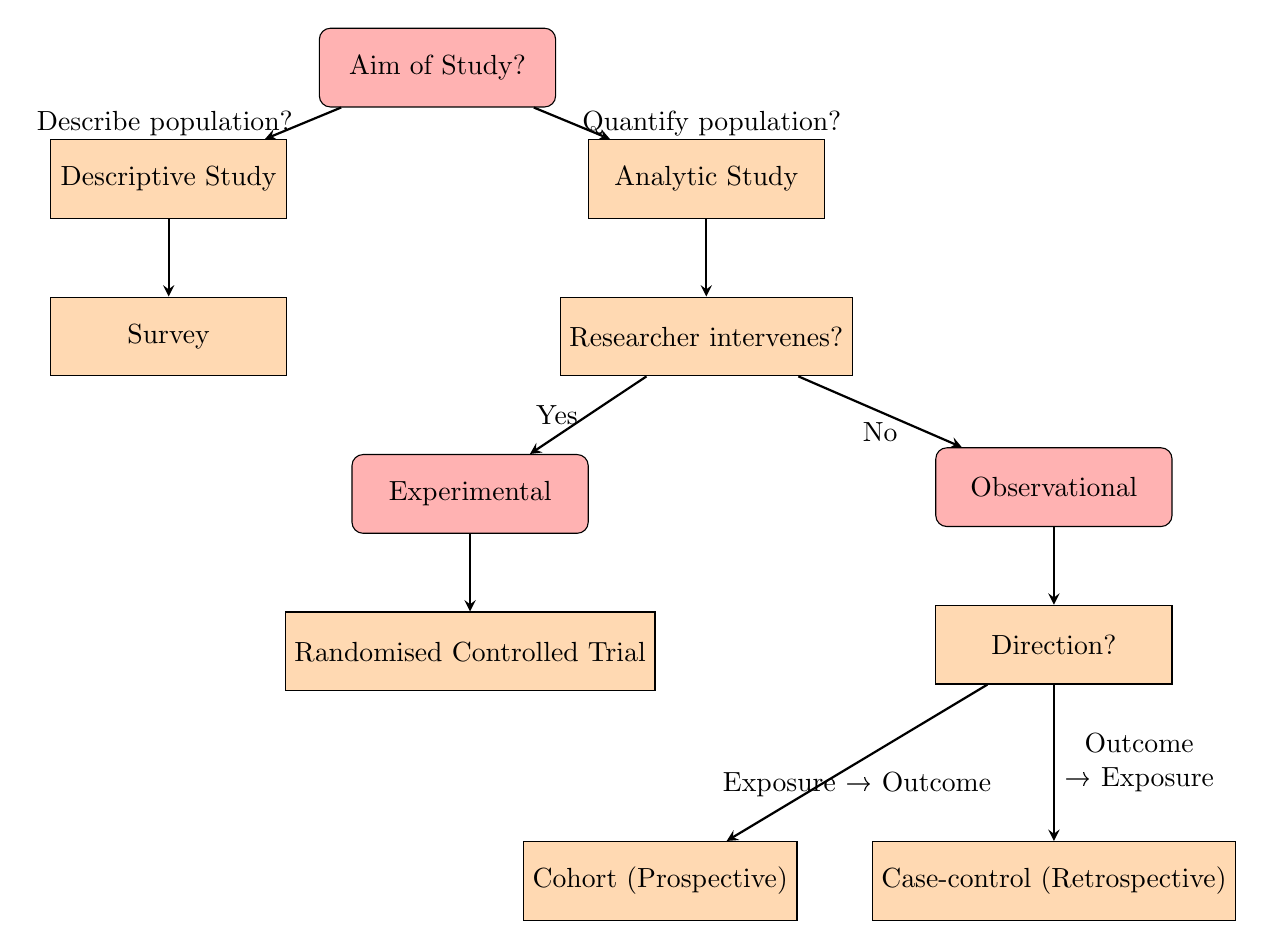
\begin{tikzpicture}[node distance=2cm]

\node (study) [startstop] {Aim of Study?};
\node (desc) [process, below left of=study, xshift=-2cm] {Descriptive Study};
\node (analytic) [process, below right of=study, xshift=2cm] {Analytic Study};
\node (survey) [process, below of=desc] {Survey};
\node (inter) [process, below of=analytic] {Researcher intervenes?};
\node (exp) [startstop, below of=inter, xshift=-3cm] {Experimental};
\node (obs) [startstop, below right of=inter, xshift=3cm, yshift=-0.5cm] {Observational};
\node (rct) [process, below of=exp] {Randomised Controlled Trial};
\node (dir) [process, below of=obs] {Direction?};
\node (cohort) [process, below of=dir, yshift=-1cm] {Case-control (Retrospective)};
\node (casecontrol) [process, left of=cohort, xshift=-3cm] {Cohort (Prospective)};

\draw [arrow] (study) -- node[anchor=east] {Describe population?}(desc);
\draw [arrow] (study) -- node[anchor=west] {Quantify population?}(analytic);
\draw [arrow] (desc) -- (survey);
\draw [arrow] (analytic) -- (inter);
\draw [arrow] (inter) -- node[anchor=east] {Yes} (exp);
\draw [arrow] (inter) -- node[anchor=north] {No} (obs);
\draw [arrow] (exp) -- (rct);
\draw [arrow] (obs) -- (dir);
\draw [arrow] (dir) -- node[anchor=west, align=center] {Outcome \\ → Exposure} (cohort);
\draw [arrow] (dir) -- node[anchor=north] {Exposure → Outcome} (casecontrol);

\end{tikzpicture}

    \begin{itemize}
    \item \textbf{Discrete}: A type of variable that can only take on specific values. These values are typically whole numbers or counts and cannot be subdivided further. For example, the number of children in a family is a discrete variable because it can only be a whole number (e.g., 1, 2, 3, etc.).
    \item \textbf{Categorical}: Represent data that falls into specific categories or groups. The categories in nominal variables do not have any inherent order or ranking. Examples of nominal variables include gender (e.g., male, female), eye colour (e.g., blue, brown, green), or types of fruit (e.g., apple, banana, orange).
    \item \textbf{Continuous}: Measurements that can take on any value within a specific range. They can be subdivided infinitely, and there are no gaps or interruptions in the possible values. Examples of continuous variables include height, weight, temperature, and time. These variables are often represented by real numbers and can include decimal values.
    \item \textbf{Ordinal}: Similar to categorical variables, but they have an inherent order or ranking associated with their categories. The order represents the relative magnitude or importance of the categories, but the actual differences between the categories may not be uniform or measurable. Examples of ordinal variables include educational attainment (e.g., high school, bachelor's, master's, Ph.D.), socioeconomic status (e.g., low, medium, high), or survey ratings (e.g., strongly agree, agree, neutral, disagree, strongly disagree).
    \item \textbf{If a data set is Categorical, must it also be Nominal?}: No. All nominal data is categorical data, but not all categorical data is nominal data. Nominal data refers specifically to categorical data without any order or hierarchy.
    \end{itemize}
\item \textbf{Types of data}


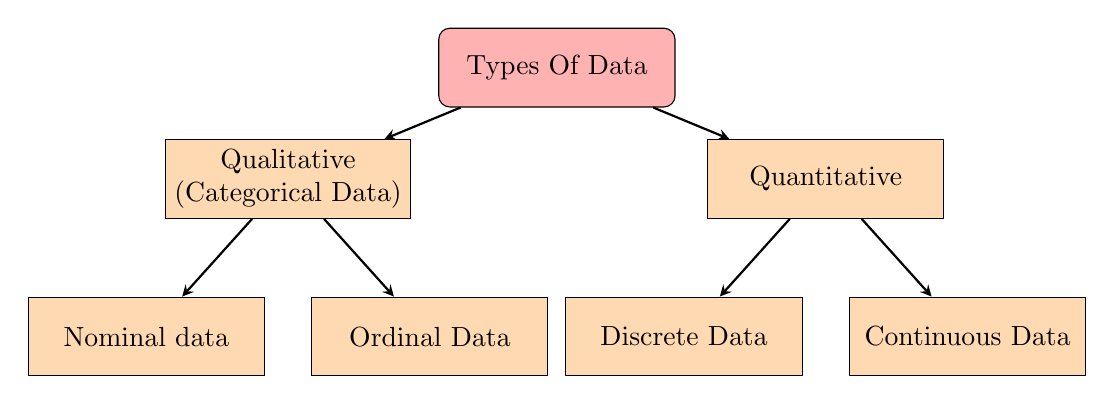
\begin{tikzpicture}[node distance=2cm]

\node (start) [startstop] {Types Of Data};
\node (cat) [process, align=center, below left of=start, xshift=-2cm] {Qualitative \\ (Categorical Data)};
\node (quant) [process, below right of=start, xshift=2cm] {Quantitative};
\node (nominal) [process, below of=cat, xshift=-1.8cm] {Nominal data};
\node (ordinal) [process, below of=cat, xshift=1.8cm] {Ordinal Data};
\node (discrete) [process, below of=quant, xshift=-1.8cm] {Discrete Data};
\node (continuous) [process, below of=quant, xshift=1.8cm] {Continuous Data};

\draw [arrow] (start) -- (cat);
\draw [arrow] (start) -- (quant);
\draw [arrow] (cat) -- (nominal);
\draw [arrow] (cat) -- (ordinal);
\draw [arrow] (quant) -- (discrete);
\draw [arrow] (quant) -- (continuous);

\end{tikzpicture}

\item \textbf{How to identify whether a study uses probability sampling?}: To find sampling frame.
\item \textbf{Note for Stratified sampling}: Stratified sampling involves dividing the population into distinct subgroups (strata) based on certain characteristics.
\item \textbf{Why Non-response can cause bias in surveys?}: because non-respondents tend to(maybe) behave differently compared to people who respond.
\end{itemize}


%%%%%%%%%%%%%%%%%%%%%%%%%%%%%%%%%%%%%%
%%%%%%%%%%%%%%%%%%%%%%%%%%%%%%%%%%%%%%
%%%%%%%%%%%%%%%%%%%%%%%%%%%%%%%%%%%%%%
%%%%%%%%CI%%%%%%%%%
%%%%%%%%%%%%%%%%%%%%%%%%%%%%%%%%%%%%%%
%%%%%%%%%%%%%%%%%%%%%%%%%%%%%%%%%%%%%%
%%%%%%%%%%%%%%%%%%%%%%%%%%%%%%%%%%%%%%
\newpage
\pagestyle{fancy}
\lhead{STAT110/115 Tutoring Materials }
\rhead{Confidence Interval}

\begin{itemize}
\item \textbf{The standard normal critical value for a 95\% interval}: 1.96
\item \textbf{Confidence interval formula}: $$\bar{x} \pm Z_{(1-\frac{\alpha}{2})} \times \frac{\sigma_X}{\sqrt{n}}$$
estimate for the mean ± multiplier ± standard error for the mean
\item \textbf{The standard normal critical value for a 99\% interval}: 2.58
\item \textbf{Multiplier formula}: $$z = \frac{x - \textbf{mean}}{\textbf{sd}}$$
\item \textbf{What is the $\alpha$ in the multiplier}: tail probability
\item \textbf{Multiplier pattern}: when CI is bigger (e.g., 95\% to 99\%), the multiplier will be bigger
\item \textbf{$s_X$}: sample standard deviation
\item \textbf{In practice the true standard deviation $\sigma_X$ is not known}: We estimate it with the sample standard deviation.
\item \textbf{This means our critical values must now come from the 't' distribution, not the standard normal}.
\item \textbf{$t$ distribution CI}: $$\bar{x} \pm t_{(1-\frac{\alpha}{2}, \nu)} \times \frac{sX}{\sqrt{n}}$$
\item \textbf{$\nu$ (degree of freedom) for t-distribution}: $\nu = n - 1$
\item \textbf{The t-distribution will be the correct sampling distribution if}: either the underlying distribution of X is normal, and/or the sample size is sufficiently large (Central Limit Theorem holds).
\item \textbf{What is the degree of freedom in t-distribution}: to replace the mean and sd in a normal distribution (because t-distribution is always standardised)
\item \textbf{When to use t-distribution}: when the sample size is small
\item \textbf{Calculate the estimate sample size when knows the CI}: assuming knows the sd and mean (normally given in the question), solve the equation, rounding UP
\item \textbf{Comparing means with CI}: $$(\bar{x}_1 - \bar{x}_2) \pm t_{(1-\frac{\alpha}{2}, \nu)} \times \sqrt{\frac{s_1^2}{n_1} + \frac{s_2^2}{n_2}}$$
\item \textbf{Using CLT to test appropriate normal distribution}: $$n\pi \pm 3 \sqrt{n\pi (1 - \pi)}$$
gives two values between 0 and n, if not, then fails the test. This approximation is good only when: n is large, $\pi$ is not close to 0 or 1 (this increases symmetry)
\item \textbf{Formula for estimating $\pi$}: $$P = \frac{X}{n}$$, $$p = \frac{x}{n}$$, x is the observed value of X. (and more) Using the Central Limit Theorem, the resulting distribution of these proportions is approximately normal if, n is large enough, $\pi$ far enough from 0 or 1. As before, we judge this using: $$n\pi \pm \sqrt{n\pi(1 - \pi)}$$ gives values between 0 and n.
\item \textbf{Derivation of the mean of the sampling distribution}: If \(P = \frac{X}{n}\), then \(\mu_P = \pi\), \textbf{sd} = \(\sigma_P = \sqrt{\frac{\pi(1 - \pi)}{n}}\)
\item \textbf{95\% confidence interval for $\pi$} (use the sample proportion (p) to estimate the unknown true population proportion ($\pi$)): $$p \pm 1.96 \sqrt{\frac{p(1 - p)}{n}}$$
\item \textbf{Margin of error}: $$multipliers * sd$$
\item \textbf{Note for CI}: This confidence interval (and margin of error) is correct only if the normal approximation to the binomial is appropriate. In practice, bias due to non-response should also be considered in our interpretation of an estimate.
\end{itemize}

%%%%%%%%%%%%%%%%%%%%%%%%%%%%%%%%%%%%%%
%%%%%%%%%%%%%%%%%%%%%%%%%%%%%%%%%%%%%%
%%%%%%%%%%%%%%%%%%%%%%%%%%%%%%%%%%%%%%
%%%%%%%%DISTRIBUTIONS%%%%%%%%%
%%%%%%%%%%%%%%%%%%%%%%%%%%%%%%%%%%%%%%
%%%%%%%%%%%%%%%%%%%%%%%%%%%%%%%%%%%%%%
%%%%%%%%%%%%%%%%%%%%%%%%%%%%%%%%%%%%%%

\newpage

\pagestyle{fancy}
\lhead{STAT110/115 Tutoring Materials }
\rhead{Distributions}
%\maketitle

\begin{itemize}
\item \textbf{Mean of the binary (Bernoulli) distribution}: $$\mu = p$$
\item \textbf{Variance of the binary (Bernoulli) distribution}: $$\sigma^2 = p (1 - p)$$
\item \textbf{Difference between binary distribution and binomial distribution}: $$n = 1 \Rightarrow binary \ distribution$$
$$n > 1 \Rightarrow binomial \ distribution$$
\textbf{Mean of the binomial distribution}:$$\mu=np$$
\textbf{Variance of the binomial distribution}:$$\sigma^2 = np(1-p)$$
\item \textbf{Conditions for binomial distribution}: Outcome is binary. We have n independent trials. The number of trials is fixed. The probability of success $\pi$ must stay constant.
\item \textbf{Probability of x successes in n trials}: $$ \Pr(X = x) = \binom{n}{x} \pi^x (1 - \pi)^{n - x} $$
\item Binomial coefficient ($\binom{n}{k}$): $$\frac{n!}{(k!)(n-k)!}$$
\textbf{Standard normal distribution(Z)}:$$Z \sim N (\mu = 0 ,\sigma^2 = 1)$$
\item \textbf{$\mu$ (normal distribution) moves the curve but does not change its shape}.
\item \textbf{$\sigma$ spreads the curve more widely about X = $\mu$ but does not alter the centre}.
\item \textbf{Compare a relative frequency histogram with a probability distribution}: Relative frequency histogram represents a sample (smaller number of individuals). The probability density function represents a population (a large number of individuals).
\item \textbf{How to estimate the value of the parameters if estimating a probability distribution curve from a relative frequency histogram}: $\mu$ is estimated by the sample mean. $\sigma$ is estimated by the sample standard deviation, s.
\item \textbf{What do the areas under the normal distribution curve represent? Probabilities}.
\item \textbf{What is Z-score (Z-value)? Number of standard deviations away from the mean}.
\item Any normal distribution value, \textbf{$X \sim N(\mu_X , \sigma^2_X)$}, can be put on the standard normal scale, \textbf{$Z \sim N(0, 1)$}. The Z-score follows a standard normal distribution.
\item \textbf{Formula for Z-Value}: $$Z = \frac{(X - \mu_X)}{\sigma_X}$$
\item \textbf{When will the sampling distribution of the mean will follow a normal distribution? If x(the samples, not X) is large enough}.
\item \textbf{Central Limit Theorem (CLT)}: The sampling distribution derived from a simple random sample will be approximately normally distributed.
\item \textbf{What is the mean of the sampling distribution? Population mean}, \textbf{$\mu_{\bar{X}} = \mu_X$}.
\item \textbf{Variance of the sampling distribution}: $$\sigma_{\bar{x}} = \frac{\sigma_x}{\sqrt{n}}$$
The variability of sample means.
\item \textbf{Notes on the sampling distribution}: If sample size n is greater, then the standard error of the mean is smaller (more compact distribution, greater precision). If X is normal, then $X_{bar}$ is normal (for any n). If X is not normal, then $X_{bar}$ is approximately normal for large n (central limit theorem).
\end{itemize}


%%%%%%%%%%%%%%%%%%%%%%%%%%%%%%%%%%%%%%
%%%%%%%%%%%%%%%%%%%%%%%%%%%%%%%%%%%%%%
%%%%%%%%%%%%%%%%%%%%%%%%%%%%%%%%%%%%%%
%%%%%%%%REGRESSION%%%%%%%%%
%%%%%%%%%%%%%%%%%%%%%%%%%%%%%%%%%%%%%%
%%%%%%%%%%%%%%%%%%%%%%%%%%%%%%%%%%%%%%
%%%%%%%%%%%%%%%%%%%%%%%%%%%%%%%%%%%%%%

\newpage

\graphicspath{{./regressionPic/}}
\pagestyle{fancy}
\lhead{STAT110/115 Tutoring Materials}
\rhead{Regression}
%\maketitle

\begin{itemize}
\item \textbf{Types of regression}: Linear (continuous data), Logistic (categorical data), Cox (categorical data in a survival analysis).
\item \textbf{Explanatory variable (X)}: Also known as a covariate, predictor, or independent variable.
\item \textbf{Outcome variable (Y)}: Also known as response or dependent variable.
\item \textbf{Simple Linear Regression (SLR)}: Looks at a relationship between two continuous variables where the relationship between the two variables is approximately a straight line.
\item \textbf{SLR equation}: $$Y = \beta_0 + \beta_1x + e$$
\begin{itemize}
\item This implies that the mean response is related to x by $$\mu_Y = \beta_0 + \beta_1x$$
\item \textbf{Y} is the numerical outcome variable (continuous or approximately so).
\item \textbf{x} is the explanatory variable.
\item \textbf{$\beta_0$} is the intercept or constant (where the line crosses the y-axis).
\item \textbf{$\beta_1$} is the slope of the line.
\item \textbf{e} (often denoted $\epsilon$) is the random error or residual term.
\end{itemize}
\item \textbf{SLR equation for estimating:}
$$\hat{y}=\hat{\beta}_0+\hat{\beta}_1x$$
\item \textbf{Residual ('estimated error') term}: $$\hat{e_i} = y_i - \hat{y_i}$$
\begin{figure}[H]
    \centering
    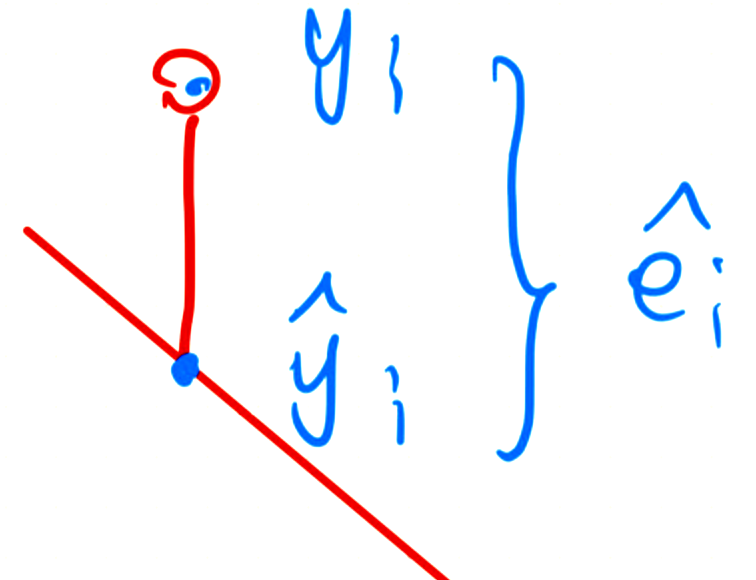
\includegraphics[width=0.2\textwidth]{92.png}
\end{figure}
\item \textbf{How to find regression line}: The line of best fit minimises the sum of the squares of the residuals.
\begin{figure}[H]
    \centering
    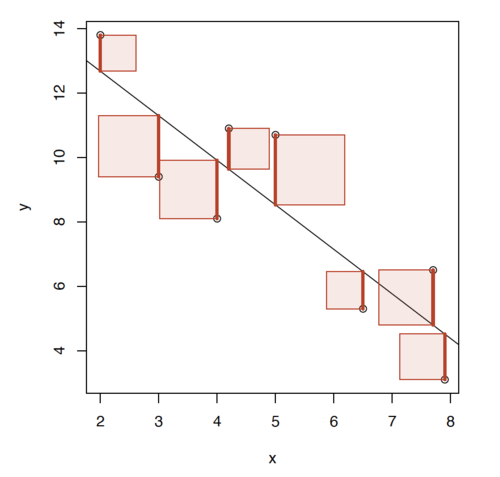
\includegraphics[width=0.3\textwidth]{1.png}
\end{figure}
\item \textbf{Equation for how to find regression line}:
$$\sum_{i=1}^{n}\hat{e}^2_i = \sum_{i=1}^{n}(y_i - \hat{y}_i )^2$$
\item \textbf{How to calculate $\beta_1$ and $\beta_0$}: 
$$\hat{\beta}_1 = \frac{\sum_{i=1}^{n}(x_i - \bar{x})(y_i - \bar{y})}{\sum_{i=1}^{n}(x_i - \bar{x})^2}$$
$$\hat{\beta}_0 = \bar{y} - \hat{\beta}_1 \bar{x}$$
\item \textbf{Example for how to calculate regression (Stress and Blood Pressure)}:
\begin{itemize}
\item Get n, n = 6
\item Find the explanatory and outcome 
\item Calculate $\beta_1$ and $\beta_0$
\item Get the regression equation
\item Using R for SLR
\end{itemize}
\item \textbf{Assumptions for Simple Linear Regression (LINE)}:
\begin{itemize}
\item Linearity: The relationship between the mean response $\mu_Y$ and x is described by a straight line.
\item Independence: The responses $Y_1,Y_2, . . . ,Y_n$ are statistically independent.
\item Normality: The error terms $e_1, e_2, . . . , e_n$ come from a normal distribution.
\item Equal variance: The error terms all have the same variance, $\sigma^2$ ('homoscedastic').
\end{itemize}
\item \textbf{What diagram is used for checking linearity}: Residual plot.
$$\hat{e}_i = y_i - \hat{y}_i = y_i - (\hat{\beta}_0 + \hat{\beta}_1 x_i) = y_i - \hat{\beta}_0 - \hat{\beta}_1 x_i$$
\item \textbf{Failure of linearity assumption}: 
\begin{figure}[H]
    \centering
    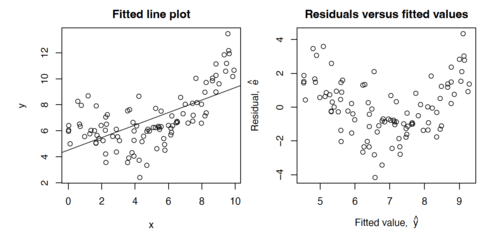
\includegraphics[width=0.7\textwidth]{2.png}
\end{figure}
\item \textbf{Linearity assumption holds}: 
\begin{figure}[H]
    \centering
    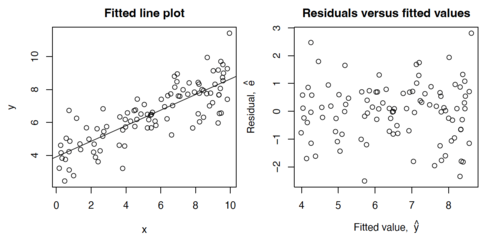
\includegraphics[width=0.7\textwidth]{3.png}
\end{figure}
\item \textbf{Checking independence assumption}: May get insight by thinking about the study design (Ask yourself questions).
\item \textbf{Plot for Checking the normality assumption}: Q - Q plot.
\item \textbf{Pass of normality assumption}: 
\begin{figure}[H]
    \centering
    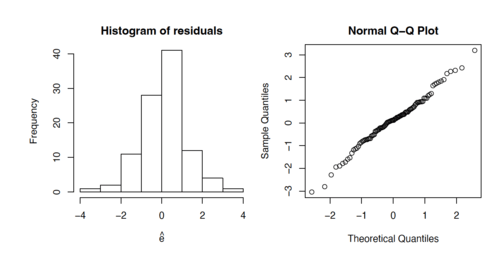
\includegraphics[width=0.7\textwidth]{4.png}
\end{figure}
\item \textbf{Fail of normality assumption}: 
\begin{figure}[H]
    \centering
    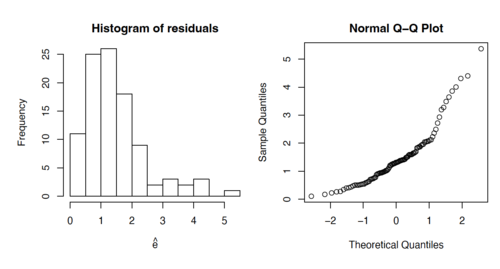
\includegraphics[width=0.7\textwidth]{5.png}
\end{figure}
\item \textbf{Checking equal variance assumption (homoscedasticity)}: Pass if the residual plot is not like this.
\begin{figure}[H]
    \centering
    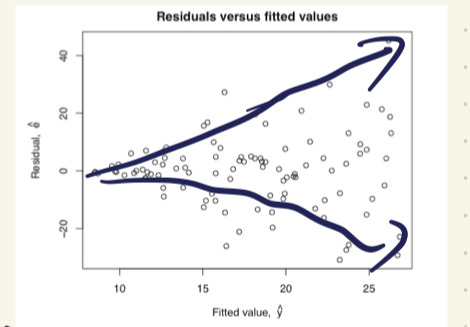
\includegraphics[width=0.5\textwidth]{6.jpg}
\end{figure}
\item \textbf{What is the impact if Fail of the linearity assumption}: Critical. If that assumption fails, all conclusions drawn from the model will be invalid.
\item \textbf{What is the impact if Fail of independence or equal variance assumptions}: Remain valid. However, estimates can be inefficient. Follows that the fitted regression line is useable. Any test results or confidence intervals based on the regression model will be invalid.
\item \textbf{What is the impact if Fail of normality assumption}: Typically least important. Effects validity of confidence intervals and test results when the sample size n is small.
\item \textbf{What to do with outliers}: The first thing to do is check that the data are correctly recorded. If data cannot be corrected, try refitting regression with outliers removed, but still investigate the cause of outliers - may be very important.
\item \textbf{Estimate of error variance}: 
$$S^2_e = \frac{1}{n-2}\sum_{i=1}^{n}(\hat{e}^2_i)=\frac{RSS}{n-2}$$
$$where \ RSS = \sum_{i=1}^{n}\hat{e}^2_i \ is \ the \ residual \ sum \ of \ squares.$$
\item \textbf{Degree of freedom for SLR's CI}: v = n - 2 because there're two parameters.
\item \textbf{What is the multiplier for SLR's CI}: 
$$t = \frac{estimate - null}{std. error}$$
\item \textbf{What is the SE for SLR's CI}:
$$s_{\hat{\beta}_1} = \frac{s_e}{\sqrt{\sum_{i=1}^{n}(x_i - \bar{x})^2}}$$
\item \textbf{Using R to find SLR's CI}: 
\begin{mdframed}[backgroundcolor=gray!15, linecolor=black]
\begin{verbatim}
> confint(model1)
                 2.5 %     97.5 %
(Intercept) 24.8300345 62.4009555
X            0.2557407  0.7284774
\end{verbatim}
\end{mdframed}
\item \textbf{$\beta_1 = 0$ indicates what}: That the response is not (linearly) related to the predictor. So the estimated slope will (almost) always be non-zero: $\hat{\beta_1} \neq 0$.
\item \textbf{Steps to test to assess the strength of evidence in the data for $\beta_1 \neq 0$}:
\begin{itemize}
\item Setting up the hypotheses: $H_0 : \beta_1 = 0$, $H_A : \beta_1 \neq 0$.
\item Calculating The test statistic
$$t = \frac{\hat{\beta}_1}{s_{\hat{\beta}_1}}$$
\item Computing the p-value
\item Draw conclusion with rejecting or not $H_0$
\end{itemize}
\item \textbf{When predicting the data}: Ignore $e_0$.
\item \textbf{Why not recommend extrapolating when predicting data}: The plot may not be linear.
\begin{figure}[H]
    \centering
    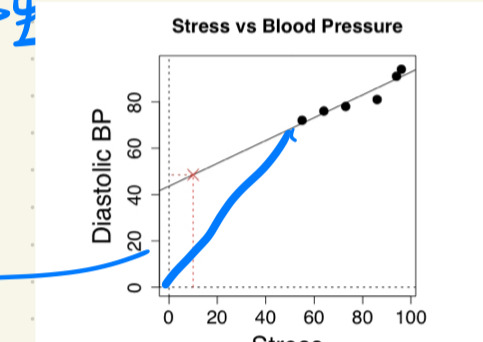
\includegraphics[width=0.4\textwidth]{7.jpg}
\end{figure}
\item \textbf{Prediction error}: The prediction error is analogous to a standard error, but takes account of both sources of uncertainty. For prediction at $x_0$, the prediction error is: 
$$PE(\hat{y}_0) = s_e\sqrt{1 + \frac{1}{n} + \frac{(x_0 - \bar{x})^2}{\sum_{i=1}^{n}(x_i - \bar{x})^2}}$$
\item \textbf{Prediction interval formula}:
$$\hat{y}_0 \pm t_{(1-\frac{\alpha}{2}, n-2)} \times PE(\hat{y}_0)$$
\item \textbf{Correlation coefficient (r)}: Summarises the strength of a linear relationship between variables. It is a measure of linear association between variables. It describes both the strength and direction of the relationship.
$$r = \frac{\sum_{i=1}^{n} (x_i - \bar{x})(y_i - \bar{y})}{\sqrt{\sum_{i=1}^{n}(x_i - \bar{x})^2 \sum_{i=1}^{n}(y_i - \bar{y})^2}}$$
\begin{itemize}
\item \textbf{r} $\in [-1, 1]$. A positive value of r means that Y and X increase together. A negative value of r means that as X increases, Y decreases (and vice-versa). 
\item The strength of the linear relationship increases as r tends towards 1 or -1. r = 0 corresponds to no linear relationship between the variables.
\end{itemize}
\item \textbf{Scatterplots for r}: 
\begin{figure}[H]
    \centering
    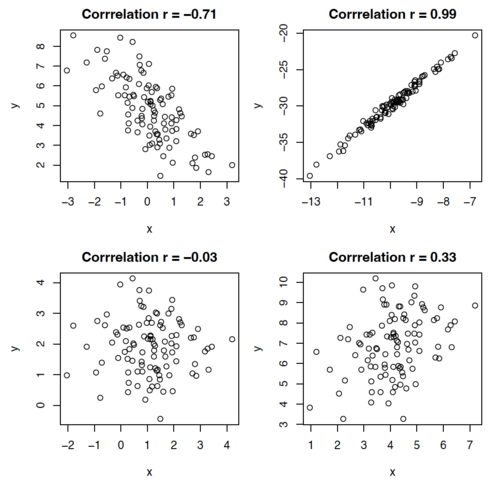
\includegraphics[width=0.7\textwidth]{8.png}
\end{figure}
\item \textbf{Re-write for r}: $s_x$ and $s_y$ are sample standard deviations for x and y variables. $s_{xy}$ is the sample covariance between x and y.
$$= \frac{S_{xy}}{S_x S_y}$$
\item \textbf{Correlation coefficient versus regression models}: The correlation coefficient is a summary of the data. Unlike linear regression, the correlation coefficient does not specify a model for the data, and cannot (for example) be used for prediction. The correlation coefficient is symmetric in the variables. That is, the correlation between x and y is the same as the correlation between y and x. In regression, the variables are not handled symmetrically. Regression models look at variation in Y for fixed values of x.
\item \textbf{Coefficient of determination ($R^2$)}: $R^2$, is a measure of how well a regression model describes the data. $R^2$ is the squared correlation between the observed and predicted responses. $R^2 \in [0, 1]$.
\item \textbf{Meaning for the value of $R^2$}: A high value of $R^2$ (close to 1) indicates a regression model that describes the data very well. Conversely, a low value of $R^2$ (close to 0) indicates a regression that describes the data poorly.
\begin{figure}[H]
    \centering
    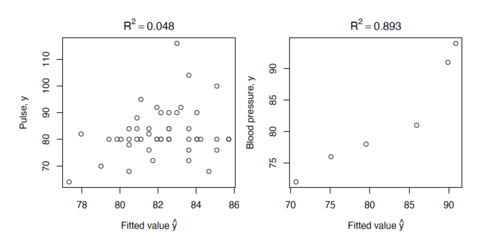
\includegraphics[width=0.7\textwidth]{9.png}
\end{figure}
\item \textbf{What describes the overall variation in the response variable?}: Total sum of squares.
$$TSS = \sum_{i=1}^{n} (y_i - \bar{y})^2$$
\item \textbf{What describes the total variation of the data points about the regression line?}: Residual sum of squares (RSS can be thought of as variation not explained by the regression model).
$$RSS = \sum_{i=1}^{n} (y_i - \hat{y}_i)^2$$
\item \textbf{What describes as the amount of variation in the response that is explained by the regression model?}: Explained sum of squares.
$$ESS = TSS - RSS$$
\item \textbf{Equation of $R^2$}: 
$$R^2 = \frac{ESS}{TSS} = 1 - \frac{RSS}{TSS}$$
\item \textbf{Correlation does not equal causation}: e.g., just because there's more ice cream in the summer and more drowning in the summer doesn't mean there's a link between ice cream and drowning.
\item \textbf{Logistic regression}: Outcome variable is binary.
\begin{figure}[H]
    \centering
    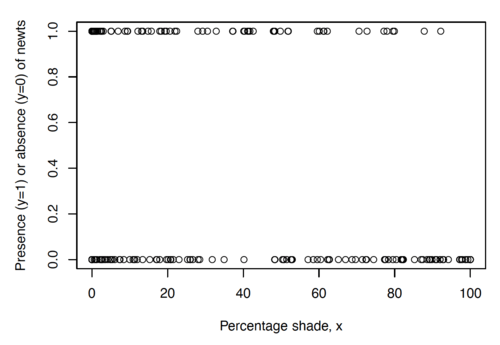
\includegraphics[width=0.5\textwidth]{91.png}
\end{figure}
\item \textbf{Equation for logistic regression}: 
$$logit(p) = \log\left(\frac{p}{1-p}\right) = \beta_0 + \beta_1x$$
$Y$ is the binary outcome variable, $Y = 1$ or $Y = 0$ for each observation. $p$ is the probability that specified category will occur; i.e. $p = Pr(Y = 1)$. $x$ is the explanatory variable. Parameters $\beta_0$, $\beta_1$ are the regression coefficients. $\beta_0$ is intercept and $\beta_1$ slope 'on the logit scale'. In the formula, log is the natural logarithm (log to base e).
\item \textbf{Which technique do we use when estimating the regression coefficients?}: Maximum likelihood estimation.
\item \textbf{What will increase x by one unit result in?}: A multiplicative change of $e^{\beta_1}$ to the odds.
\item \textbf{Formula for logistic curve for the probability p}: 
$$p = \frac{e^{\beta_0 + \beta_1x}}{1+e^{\beta_0 + \beta_1x}}$$
\item \textbf{Testing in logistic regression}:
\begin{itemize}
\item Define the hypotheses: $H_0 : \beta_1 = 0$ and $H_A : \beta_1 \neq 0$.
\item The test statistic is: 
$$z = x\frac{\hat{\beta}_1}{s_{\hat{\beta}_1}}$$
\item Get the corresponding p-value.
\item Reject/not reject $H_0$.
\item Conclusion.
\end{itemize}
\item \textbf{Multiple regression model}:
$$Y = \beta_0 + \beta_1x_1 + \cdots + \beta_kx_k + e$$
\item \textbf{Mean value of the Multiple regression model}: 
$$\mu_Y = \beta_0 + \beta_1x_{1} + \cdots + \beta_kx_{k}$$
\item \textbf{Applications of multiple regression}:
\begin{itemize}
\item Adjusting for the effect of confounding variables.
\item Establishing which variables are important in explaining the values of the response variable.
\item Predicting values of the response variable.
\item Describing the strength of the association between the response variable and the explanatory variables.
\end{itemize}
\item \textbf{Least squares estimates}: 
$$\sum_{i=1}^{n} (y_i - \hat{y}_i)^2$$
\item \textbf{RSS for $\hat{e_i}$}: 
$$RSS = \sum_{i=1}^{n} \hat{e}_i^2$$
To estimate the error variance $\sigma^2_e$.
\item \textbf{Usual estimate}: 
$$s_e^2 = \frac{RSS}{n - k - 1}$$
\end{itemize}

%%%%%%%%%%%%%%%%%%%%%%%%%%%%%%%%%%%%%%
%%%%%%%%%%%%%%%%%%%%%%%%%%%%%%%%%%%%%%
%%%%%%%%%%%%%%%%%%%%%%%%%%%%%%%%%%%%%%
%%%%%%%%HYPOTHESIS TESTING%%%%%%%%%
%%%%%%%%%%%%%%%%%%%%%%%%%%%%%%%%%%%%%%
%%%%%%%%%%%%%%%%%%%%%%%%%%%%%%%%%%%%%%
%%%%%%%%%%%%%%%%%%%%%%%%%%%%%%%%%%%%%%

\newpage

\pagestyle{fancy}
\lhead{STAT110/115 Tutoring Materials }
\rhead{Hypothesis Testing}
%\maketitle

\begin{itemize}
\item \textbf{$H_0$}: Null hypothesis. The hypothesis is that there is no association, no effect or no difference.
\item \textbf{$H_A$}: Alternative hypothesis. The hypothesis is that there is an association, effect or difference.
\item \textbf{P-value}: We measure the "consistency" of the observed data with the claim using a p-value. The p-value is the probability of observing the value of the test statistic, or a value more extreme, calculated under the assumption that $H_0$ is true. A small p-value indicates we would be unlikely to see the data we did if the null hypothesis were true. i.e., the smaller the p-value is, the easier to reject $H_0$. If the p-value is less than $\alpha$ we reject $H_0$. If the p-value is greater than or equal to $\alpha$ we do not reject $H_0$.
\item \textbf{Test statistic (t - statistic)}: A test statistic is the standardised value of the sample value. 
$$T = \frac{observed \ sample \ value - null \ value}{estimated \ standard \ error}$$
When studying hypothesis testing, we usually use $\pi$ to denote the value of the overall parameter, instead of using p.
\item \textbf{Z Statistic vs t-statistic}:
\begin{itemize}
\item Z-statistic: When to use: Large samples (n $>$ 30) or known population standard deviation ($\sigma$). Basis: Uses population standard deviation ($\sigma$).
\item t-statistic: When to use: Small samples (n $<$ 30) or unknown population standard deviation ($\sigma$). Basis: Uses sample standard deviation (s).
\end{itemize}
\item \textbf{How to conduct a hypothesis test}:
\begin{enumerate}
\item Set $H_0$ and $H_A$.
\item Calculate t-statistic(if it is sample) or Z-statistic(if it is population).
\item Calculate p-value.
\item Calculate 95\% CI with (3).
\item Draw a conclusion based on the p-value (reject $H_0$ or not).
\end{enumerate}
\item \textbf{The difference between p and p*}:
\begin{itemize}
\item p (Sample Proportion): Frequency or proportion of events in a sample. Example: If 50\% support a policy in a sample, ( p = 0.5 ).
\item p* (Estimate of Overall Proportion): Estimate of the overall proportion based on sample data. Example: If 50\% support a policy in a sample, ( p* = 0.5 ).
\end{itemize}
\item \textbf{When to use chi square}: When trying to control groups in experiments - looking for differences between men and women in each group, etc. Looking for differences between categorical variables - maybe you want to know if there is a difference between men and women for their favourite type of ice cream.
\item \textbf{How to conduct chi-square test}:
\begin{enumerate}
\item Define the Null-Hypothesis and Alternative Hypothesis. $H_0$ : The treatment and response are independent (i.e. no association). $H_A$ : The treatment and response are dependent in some way (i.e. there is some association).
\item Calculating expected cell counts.
\item Calculating the $\chi^2$ test statistic.
\item Get the degree of freedom.
\item Calculate the p-value with R.
\item Reject / not reject $H_0$.
\item Draw conclusion.
\end{enumerate}
\item \textbf{Expected cell counts}: 
$$E_{(row \ i, col \ j)} = \frac{r_i \times c_j}{n}$$
\begin{itemize}
\item $r_i$ is the row total, for row i
\item $c_j$ is the column total, for column j 
\item n is the total number (of trials, patients, etc.)
\end{itemize}
We worked out what we would have expected to see under the null hypothesis in each cell given the observed row and column totals.
\item \textbf{Formula for chi-square:}
$$\chi^2=\sum_{ij}\frac{(O_{ij}-E_{ij})^2}{E_{ij}}$$
\item \textbf{Degree of freedom for chi square}: $\nu = (number of rows - 1) * (number of columns - 1)$
\item \textbf{Range for p-value}: (0, 1)
\item \textbf{Belief (interpretation/decision):}
\begin{table}[h!]
\centering
\begin{tabular}{|l|c|c|}
\hline
& Fail to reject $H_0$ & Reject $H_0$ \\ \hline
Null is true & Correct interpretation (No error) & Error (Type I) \\ \hline
Null is false & Error (Type II) & Correct interpretation (No error) \\
\hline
\end{tabular}
\end{table}
\item \textbf{Type I error (a false positive result)}: Concluding that there is an association between exposure and outcome, where there is not. Type I error is controlled when we set the significance level (usually 0.05).
\item \textbf{Type II error (a false negative result)}: Concluding that there is not an association between exposure and outcome, where there is. Type II error is primarily controlled through the sample size. Ideally, power should be between 80 and 90\%.
\end{itemize}

\graphicspath{{./}}


%%%%%%%%%%%%%%%%%%%%%%%%%%%%%%%%%%%%%%
%%%%%%%%%%%%%%%%%%%%%%%%%%%%%%%%%%%%%%
%%%%%%%%%%%%%%%%%%%%%%%%%%%%%%%%%%%%%%
%%%%%%%%ANOVA%%%%%%%%%
%%%%%%%%%%%%%%%%%%%%%%%%%%%%%%%%%%%%%%
%%%%%%%%%%%%%%%%%%%%%%%%%%%%%%%%%%%%%%
%%%%%%%%%%%%%%%%%%%%%%%%%%%%%%%%%%%%%%
\newpage

\pagestyle{fancy}
\lhead{STAT110/115 Tutoring Materials}
\rhead{ANOVA}

\begin{itemize}
\item \textbf{ANOVA}: Abbreviation of \textbf{Analysis of Variance}.
\item \textbf{Methods for comparing means} of continuous responses between multiple groups.
\item \textbf{F-ratio}: Signal/noise
\begin{figure}[H]
    \centering
    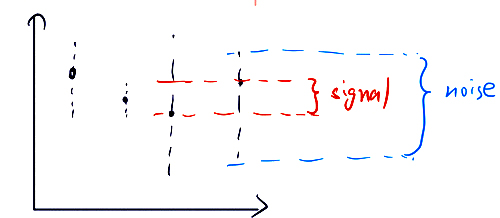
\includegraphics[width=0.4\textwidth]{anova.jpg}
\end{figure}
\item \textbf{Reasons why using "2+2+2=3" is undesirable}:
    \begin{itemize}
    \item It's more work than we need to do. Three tests may not seem too bad, but to compare 10 groups we would have to do 45 different pairwise t-tests.
    \item It can lead to lots of false positive results. Every test has the potential to incorrectly reject H0; i.e. falsely identify a difference between a pair of groups. If we do lots of tests then we risk generating lots of false positives.
    \end{itemize}
\item \textbf{ANOVA model}: 
$$Y_{ij}=\mu_i+e_{ij}$$
$\mu_i$ is the true mean response for the ith group at the population level. $e_{ij}$ is the error term for the jth response in the ith group. The error terms are assumed to be independent and to follow a N(0, $\sigma^2$) with constant variance. The number of different groups is denoted K, and the number of responses in the ith group is denoted $n_i$.
\item \textbf{Est. mean for ANOVA}: The "." = est. Value.
$$\hat{\mu}_i = \bar{y}_i.$$
\item \textbf{Sample mean for the ith group:}
$$\bar{y}_i.=\frac{1}{n_i}\sum_{j=1}^{n}y_{ij}$$
\item \textbf{Formula for residual sum of squares in ANOVA} (no need to memorise):
$$RSS=\sum_{i=1}^{K}\sum_{j=1}^{n_i}(y_{ij}-\hat{\mu}_i)^2=\sum_{i=1}^{K}\sum_{j=1}^{n_i}(y_{ij}-\bar{y}_i.)^2$$
\item \textbf{Total sum of squares in ANOVA} (no need to memorise):
$$TSS=\sum_{i=1}^{K}\sum_{j=1}^{n_i}(y_{ij}-\bar{y}..)^2$$
\item \textbf{$y..$} is the sample mean overall the data.
\item \textbf{Formula for GSS in ANOVA} (no need to memorise): 
$$GSS = TSS - RSS$$ 
$$GSS = \sum_{i=1}^{k}n_i(\bar{y}_i.-\bar{y}..)^2$$
GSS can be interpreted as a measure of the variation that is explained by differences between groups.
\item \textbf{Setting up the hypotheses to test ANOVA:}

As usual, the null hypothesis will be the 'no difference' hypothesis:
$$H_0: \mu_1=\mu_2=...=\mu_K$$
The alternative is simply an expression that the null is incorrect:

\centerline {$H_A:\mu_1, \mu_2, ..., \mu_K$ not all equal.}

\item \textbf{Equation for F statistic:}
$$F = \frac{GSS/(K-1)}{RSS/(n-K)}$$
\item \textbf{GMS}: GSS/(K - 1) is the group mean square.
\item \textbf{RMS}: RSS/(n - K) is the residual mean square.
\item \textbf{What situations would let $H_0$ fail}: Large differences between group means. Relatively large value of GSS. A large value of F.
\item \textbf{ANOVA table:}
\begin{table}[h]
\centering
\begin{tabular}{lccc}
\hline
Source & SS & DF & MS \\ \hline
Groups & GSS & $K - 1$ & $\frac{GSS}{K - 1}$ \\
Residuals & RSS & $n - K$ & $\frac{RSS}{n - K}$ \\ \hline
Total & TSS & $n - 1$ \\ \hline
\end{tabular}
\end{table}
\item \textbf{P-value is right censored}.
\item \textbf{Blocking variable}: A second treatment variable that when included in ANOVA analysis will have the effect of reducing the SSE term (noise).
\end{itemize}

\newpage
\thispagestyle{empty}
\mbox{}
\newpage


\end{document}